\documentclass{estilo}

\usepackage{multicol}
\usepackage{enumitem}
\usepackage{graphicx}
\usepackage{float}
\usepackage{amsmath}        % para los vectores columnas
\usepackage{amsmath}



\usepackage{listings}
\usepackage{xcolor}
\definecolor{codegreen}{rgb}{0,0.6,0}
\definecolor{codegray}{rgb}{0.5,0.5,0.5}
\definecolor{codepurple}{rgb}{0.58,0,0.82}
\definecolor{backcolour}{rgb}{0.95,0.95,0.92}
\lstdefinestyle{mystyle}{
    backgroundcolor=\color{backcolour},   
    commentstyle=\color{codegreen},
    keywordstyle=\color{magenta},
    numberstyle=\tiny\color{codegray},
    stringstyle=\color{codepurple},
    basicstyle=\ttfamily\footnotesize,
    breakatwhitespace=false,         
    breaklines=true,                 
    captionpos=b,                    
    keepspaces=true,                 
    numbers=left,                    
    numbersep=5pt,                  
    showspaces=false,                
    showstringspaces=false,
    showtabs=false,                  
    tabsize=2
}
\lstset{style=mystyle}


\begin{document}

\maketitle

\section*{Enunciado}
Dada la transferencia
$$
H(s) = \frac{0.8911 s^4}{s^4 + 2539 s^3 + 4.686 \cdot 10^6 s^2 + 2.894 \cdot 10^9 s + 2.863 \cdot 10^{12}}
$$

\begin{enumerate}
    \item[\hyperlink{ej1}{1.}] Definir el tipo de filtro y calcular los polos y los ceros de $H(s)$. En el caso que corresponda calcule los parámetros $\omega_0$, $Q$ y la ganancia de la misma.
    \item[\hyperlink{ej2}{2.}] Realizar el cálculo analítico de las respuestas al impulso, al escalón y al seno (en 1 frecuencia) y graficar.
    \item[\hyperlink{ej3}{3.}] Elegir un circuito con amplificadores operacionales que cumpla con la transferencia propuesta. Justificar la elección del mismo.
    \item[\hyperlink{ej4}{4.}] Definir los valores de los componentes, normalizando según se indica. Recalcular la transferencia con los valores normalizados.
        \begin{itemize}
            \item Capacitores: utilizar la serie del 10\% (E24) y valores entre $1 n F$ y $1 \mu F$
            \item Resistores: utilizar la serie del 1\% (E96) o 5\% (E48) y valores entre $1k\Omega$ y $1M\Omega$
        \end{itemize}
    \item[\hyperlink{ej5}{5.}] Calcular el error porcentual de los parámetros $\omega_0$, $Q$, la ganancia y las singularidades del sistema respecto a la transferencia original.
    \item[\hyperlink{ej6}{6.}] Realizar las simulaciones \textit{a}, \textit{b}, \textit{c}, \textit{d} y \textit{e}. Tanto para la transferencia original como para la transferencia con los valores normalizados.
    \item[\hyperlink{ej7}{7.}] Realizar las simulaciones \textit{a}, \textit{b}, \textit{d} y \textit{e} para el filtro con Spice.
\end{enumerate}
Simulaciones:
    \begin{enumerate}[label=\alph*)]
        \item Diagramas de Bode de módulo y fase
        \item Respuesta al escalón
        \item Respuesta al impulso
        \item Respuesta a señal senoidal (3 frecuencias características)
        \item Respuesta a señal cuadrada de frecuencias: $f_o/10$,  $f_o$ y $10\cdot f_o$
    \end{enumerate}

\newpage

\tableofcontents

\newpage 

\section*{Aclaraciones}
Todas los gráficos y simulaciones de circuitos fueron realizados en MatLab.\\
\vskip0.5cm
Los análisis cualitativos de las respuestas se harán en el ítem 6 y no en el ítem 2.\\
\vskip0.5cm
Se utilizó la serie E24 para capacitores y E96 para resistencias.

\newpage 

\hypertarget{ej1}{\section{Tipo de filtro}}
\subsection{Análisis de límites}
Para analizar de qué tipo de filtro se trata según la transferencia se calculan los límites para H de s tendiendo a 0 y tendiendo a infinito.

\begin{minipage}{\linewidth}
  \centering
  \begin{minipage}{0.45\linewidth}
    $$\lim_{s \rightarrow 0} H(s) = 0$$
  \end{minipage}
  \hspace{0.05\linewidth}
  \begin{minipage}{0.45\linewidth}
    $$\lim_{s \rightarrow \infty} H(s) = 0.8911$$
  \end{minipage}
\end{minipage}
\vskip0.5cm

Por lo que se concluye que se trata de un filtro pasa altos, pues para las frecuencias cercanas a 0 la ganancia tiende a 0, mientras que para frecuencias altas (tendiendo a infinito) la ganancia es distinta de 0. 

\subsection{Análisis de polos y ceros}
La función de transferencia posee un único cero para $s=0$ y este se trata de un cero de orden 4.

Analizando el denominador se obtiene que la función de transferencia tiene los siguientes polos:
$$
p_{1, 2} = -1136.16 \pm 1374.31 j
$$
$$
p_{3, 4} = -133.34 \pm 939.50 j
$$

Dichos valores se visualizarán en el siguiente diagrama de polos y ceros.

\begin{figure}[H]
    \centering
    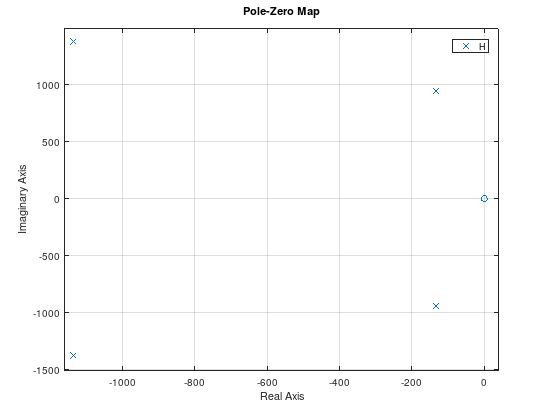
\includegraphics[width=1\textwidth]{resources/pzmap.png}
    \caption{Diagrama de polos y ceros para el circuito}
\end{figure}

Sabiendo esto, podemos descomponer el filtro en dos.

\begin{align*}
    H(s) & = 0.8911 \cdot \frac{s^2}{(s-p_1)\cdot(s-p_2)} \cdot \frac{s^2}{(s-p3)\cdot(s-p4)} \\
         & = \frac{K_1 s^2}{s^2 + 2272.32s+3.17959\cdot10^6} \cdot \frac{K_2 s^2}{s^2+266.68s+900440} \\\\
         & = H_1(s) \cdot H_2(s)
\end{align*}
Con $K_1\cdot K_2 = 0.8911$
\vskip0.5cm
Teniendo en cuenta que los polos denominadores de nuestra transferencia son de la forma  \\$s^2+\frac{\omega_o}{Q}s+\omega_o^2$, se calculará para cada transferencia $H_1$ y $H_2$ cada factor. Siendo entonces:

\begin{itemize}
    \centering
    \item[$H_1$:  ] $\omega_o = 1783.14 $ y $Q = 0.7847$ 
    \item[$H_2$:  ] $\omega_o = 948.91$ y $Q = 3.5583$
\end{itemize}

Ambos valores de Q tienen sentido pues en ambos filtros estamos en presencia de polos complejos conjugados.

\subsection{Análisis de la frecuencia de corte} 
Dado que estamos frente a un filtro pasa altos es oportuno calcular la frecuencia de corte del filtro, es decir la frecuencia $f_o = \frac{\omega_o}{2 \pi}$ tal que la señal se ha atenuado $3dB$, esto es equivalente a que la ganancia máxima se ha reducido en un $29.3\%$. Veamos gráficamente

\begin{figure}[H]
    \centering
    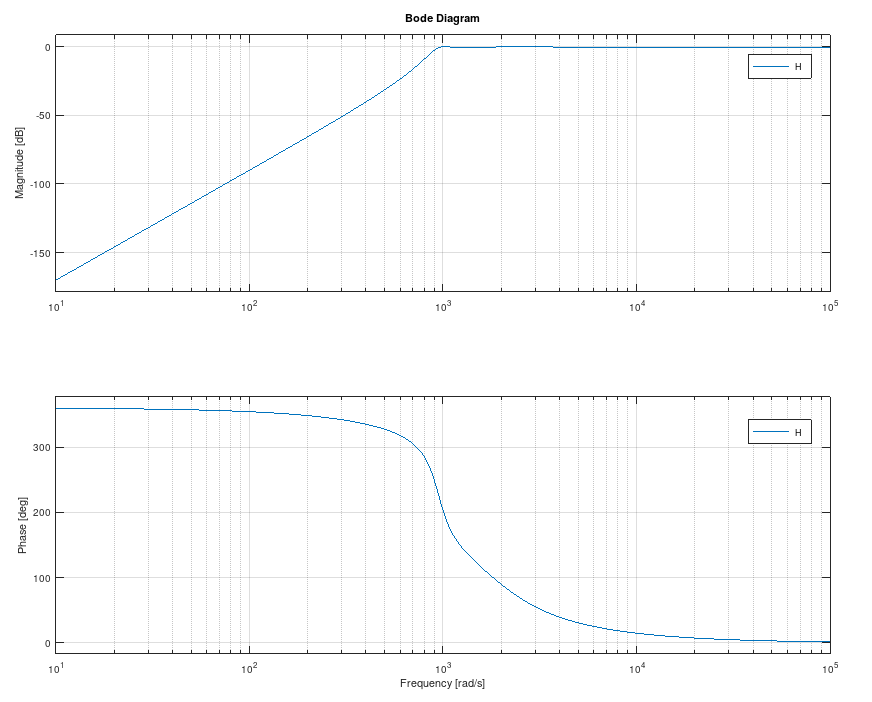
\includegraphics[width=0.8\textwidth]{resources/Bode.png}
    \caption{Diagrama de Bode. En el eje horizontal está la frecuencia angular $\omega$}
\end{figure}

Resolviendo numéricamente (utilizando la biblioteca de sympy en python3) se obtiene el valor para $\omega_o = 895.3 rad/s$, esto se traduce en una frecuencia de corte $f_o = \frac{\omega_o}{2\pi} = 142.4Hz$

\hypertarget{ej2}{\section{Cálculo analítico de las respuestas}}
\subsection{Respuesta al impulso}
Cuando $v_i(t) = \delta(t), V_i(s) = 1$. Por lo tanto, basta con calcular la transformada inversa de Laplace de $V_o(s) = H(s)$. Para ello se procede a realizar fracciones simples de $V_o(s)$
$$
V_o(s) = \frac{A}{s-p_1} + \frac{B}{s-p_2} + \frac{C}{s-p_3} + \frac{D}{s-p_4}
$$
\vskip0.5cm
Donde:
$$
A = Res(V_o(s), p_1) = \frac{0.8911 p_1^4}{(p_1-p_2)(p_1-p_3)(p_1-p_4)} = -1105 + 439j
$$
$$
B = Res(V_o(s), p_2) = \frac{0.8911 p_2^4}{(p_2-p_1)(p_2-p_3)(p_2-p_4)} = -1105 - 439j
$$
$$
C = Res(V_o(s), p_3) = \frac{0.8911 p_3^4}{(p_3-p_1)(p_3-p_2)(p_3-p_4)} = -26 - 137j
$$
$$
D = Res(V_o(s), p_4) = \frac{0.8911 p_4^4}{(p_4-p_1)(p_4-p_2)(p_4-p_3)} = -26 + 137j
$$
\vskip0.5cm
Por otro lado, tenemos que $\mathcal{L}^{-1}(\frac{1}{s-a}) = e^{at}$, por lo que resulta que:
$$
v_o(t) = A \cdot e^{p_1t} + B \cdot e^{p_2t} + C \cdot e^{p_3t} + D \cdot D e^{p_4t}
$$
\vskip0.5cm
Y como $ A = \overline{B}$, $C = \overline{D}$ y además $p_1 = \overline{p_2}$, $p_3 = \overline{p_4}$, entonces se tiene que:
$$
v_o(t) = 2\Re(A \cdot e^{p_1t}) + 2\Re(C \cdot e^{p_3 t})
$$
\vskip0.5cm
Por lo tanto se obtiene:
\begin{align*}
    v_o(t) & = -2210.14 cos(1374.31t)e^{-1136.16t} -878.06sen(1374.31t)e^{-1136.16t}\\
           & + -52 cos(939.5t) e^{-133.34t} + 274 sen(939.5t)e^{-133.34t}
\end{align*}

\begin{figure}[H]
    \centering
    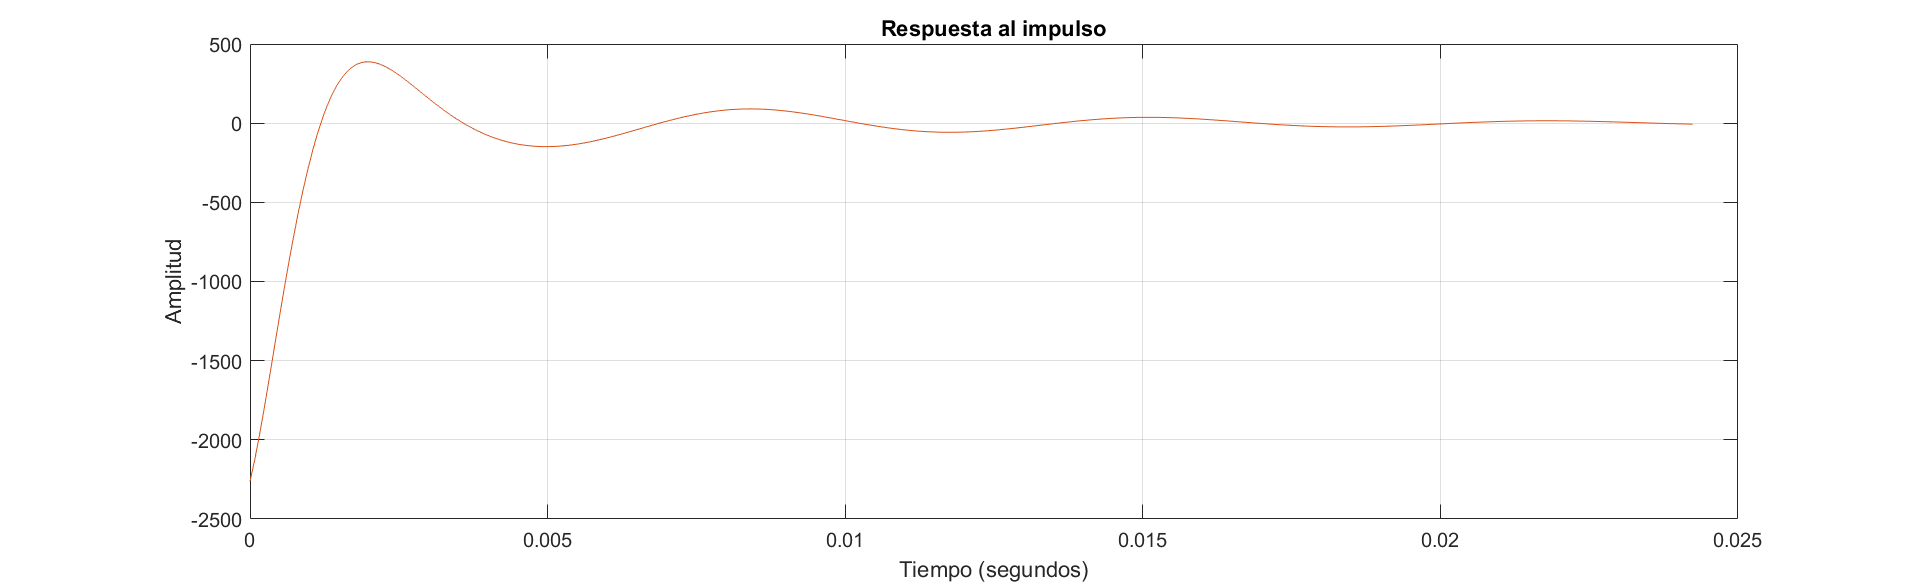
\includegraphics[width=1\textwidth]{resources/RespuestaAlImpulso.png}
    \caption{Respuesta al impulso}
\end{figure} 

\subsection{Respuesta al escalón}
Cuando $v_i(t) = \Delta(t)$, siendo $\Delta(t)$ la función escalón de Heaviside, entonces se tiene que $V_i(s) = \frac{1}{s}$. Por lo tanto, basta con calcular la transformada inversa de Laplace de
$$
V_o(s) = \frac{1}{s} H(s) = \frac{0.8911 s^3}{s^4 + 2539 s^3 + 4.686 \cdot 10^6 s^2 + 2.894 \cdot 10^9 s + 2.863 \cdot 10^{12}}$$
\vskip0.5cm
Para ello se procede a realizar fracciones simples de $V_o(s)$

$$
V_o(s) = \frac{A}{s-p_1} + \frac{B}{s-p_2} + \frac{C}{s-p_3} + \frac{D}{s-p_4}
$$
\vskip0.5cm
Donde:
$$
A = Res(V_o(s), p_1) = \frac{0.8911 p_1^3}{(p_1-p_2)(p_1-p_3)(p_1-p_4)} = 0.5846 + 0.3208j
$$
$$
B = Res(V_o(s), p_2) = \frac{0.8911 p_2^3}{(p_2-p_1)(p_2-p_3)(p_2-p_4)} = 0.5846 - 0.3208j
$$
$$
C = Res(V_o(s), p_3) = \frac{0.8911 p_3^3}{(p_3-p_1)(p_3-p_2)(p_3-p_4)} = -0.1391 + 0.0476j
$$
$$
D = Res(V_o(s), p_4) = \frac{0.8911 p_4^3}{(p_4-p_1)(p_4-p_2)(p_4-p_3)} = -0.1391 - 0.0476j
$$
\vskip0.5cm
Por lo tanto,

\begin{align*}
    v_o(t) & = 1.1692cos(1374.31t)e^{-1136.16t} - 0.6416sen(1374.31t)e^{-1136.16t}\\
           & + -0.2782cos(939.5t)e^{-133.34t} -0.094sen(939.5t)e^{-133.34t}
\end{align*}

\begin{figure}[H]
    \centering
    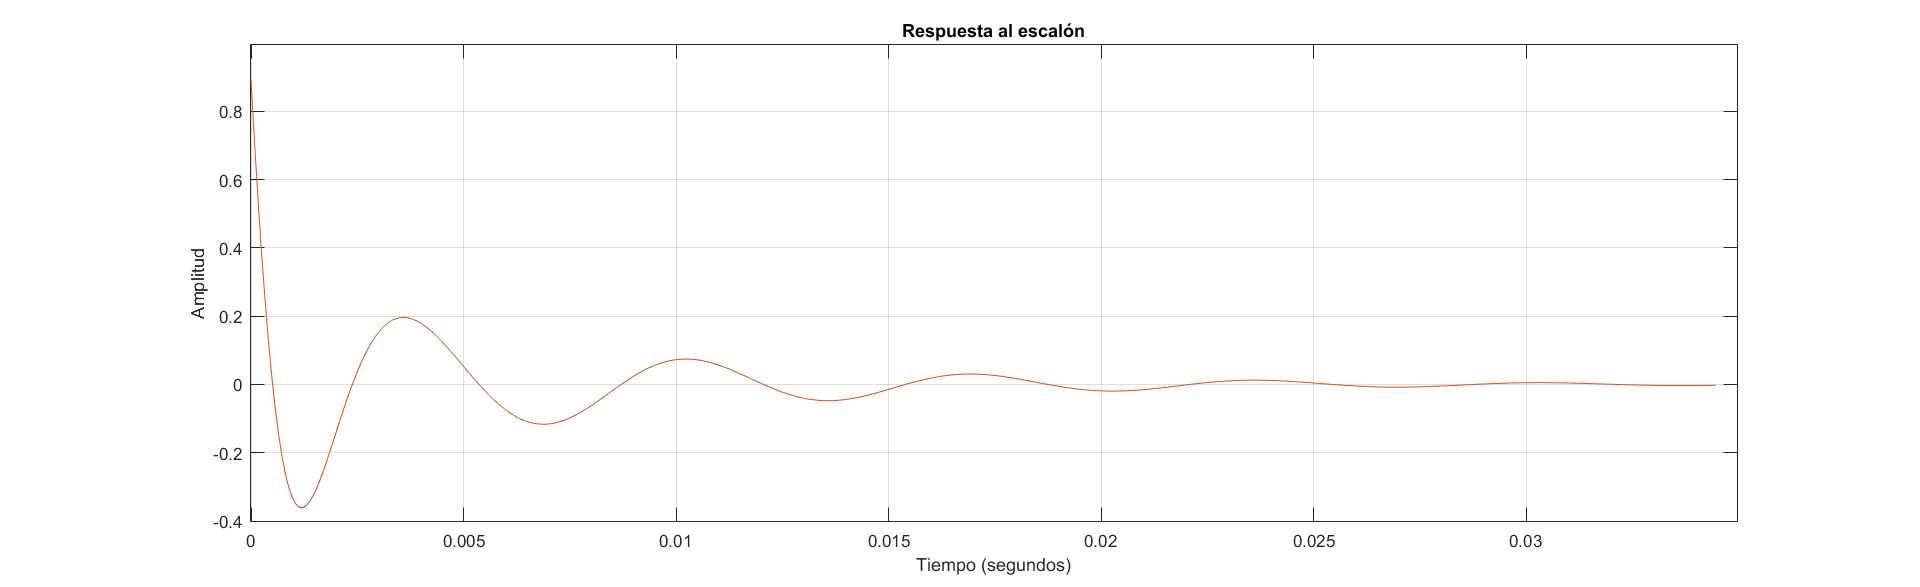
\includegraphics[width=1\textwidth]{resources/RespuestaAlEscalon.png}
    \caption{Respuesta al escalón}
\end{figure}


\subsection{Respuesta a la señal sinusoidal (frecuencia de corte)}
Dado que $\mathcal{L}(sen(\omega t)) = \frac{\omega}{\omega^2+s^2}$, y tomando $\omega = \omega_0 = 895.3 \frac{rad}{s}$. Para obtener la salida del filtro será necesario realizar la transformada inversa de Laplace de

$$
    V_o = \frac{895.3}{895.3^2+s^2} \cdot H(s) = \frac{797.8 s^4}{(s^4 + 2539 s^3 + 4.686 \cdot 10^6 s^2 + 2.894 \cdot 10^9 s + 2.863 \cdot 10^{12})(s^2+895.3^2)}
$$

Ahora, los polos serán:
$$
    p_1 = -1136.16 + 1374.31j
$$
$$
    p_2 = -1136.16 - 1374.31j
$$
$$
    p_3 = -133.34 + 939.50j
$$
$$
    p_4 = -133.34 - 939.50j
$$
$$
    p_5 = 895.3j
$$
$$
    p_6 = -895.3j
$$
\vskip0.5cm
Por lo tanto:
\vskip0.5cm
$$
V_o(s) = \frac{A}{s-p_1} + \frac{B}{s-p_2} + \frac{C}{s-p_3} + \frac{D}{s-p_4} + \frac{E}{s-p_5} + \frac{F}{s-p_6}
$$
\vskip0.5cm
Siendo los coeficientes:
\vskip0.5cm
$$
A = Res(V_o(s), p_1) = \frac{797.8 p_1^4}{(p_1-p_2)(p_1-p_3)(p_1-p_4)(p_1-p_5)(p_1-p_6)} = -0.1459 - 0.3073j
$$
$$
B = Res(V_o(s), p_2) = \frac{797.8 p_2^4}{(p_2-p_1)(p_2-p_3)(p_2-p_4)(p_2-p_5)(p_2-p_6)} = -0.1459 + 0.3073j
$$
$$
C = Res(V_o(s), p_3) = \frac{797.8 p_3^4}{(p_3-p_1)(p_3-p_2)(p_3-p_4)(p_3-p_5)(p_3-p_6)} = 0.4825 + 0.0284j
$$
$$
D = Res(V_o(s), p_4) = \frac{797.8 p_4^4}{(p_4-p_1)(p_4-p_2)(p_4-p_3)(p_4-p_5)(p_4-p_6)} = 0.4825 - 0.0284j
$$
$$
E = Res(V_o(s), p_5) = \frac{797.8 p_5^4}{(p_5-p_1)(p_5-p_2)(p_5-p_3)(p_5-p_4)(p_5-p_6)} = -0.3365 + 0.1097j
$$
$$
F = Res(V_o(s), p_6) = \frac{797.8 p_6^4}{(p_6-p_1)(p_6-p_2)(p_6-p_3)(p_6-p_4)(p_6-p_5)} = -0.3365 - 0.1097j
$$
\vskip0.5cm
Y nuevamente por propiedades de números complejos conjugados:
\vskip0.5cm
$$
    v_o(t) = 2\Re(Ae^{p_1t}) + 2\Re(Ce^{p_3t}) + 2\Re(Ee^{p_5t})
$$
\vskip0.5cm

\begin{align*}
    v_o(t) & = e^{-1136.16t} \cdot (-0.2918 \cdot cos(1374.31t) + 0.6146 \cdot sen(1374.31t)) \\
           & + e^{-133.34t} \cdot (0.965 \cdot cos(939.5t) - 0.0568 \cdot sen(939.5t)) \\
           & - 0.673 \cdot cos(895.3t) - 0.2194 \cdot sen(895.3t)
\end{align*}

\begin{figure}[H]
    \centering
    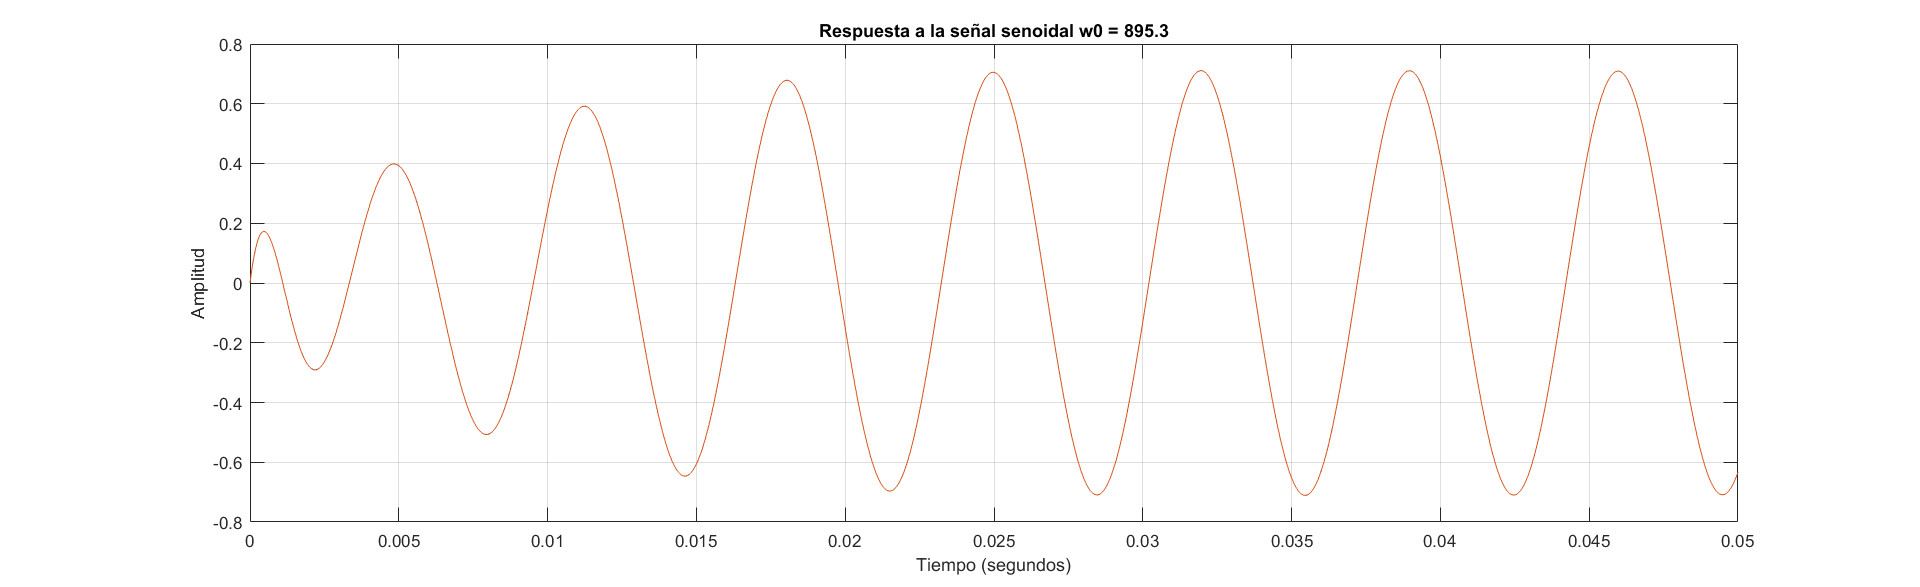
\includegraphics[width=1\textwidth]{resources/RespuestaAlSinusoide.png}
    \caption{Respuesta a la señal senoidal}
\end{figure}

\hypertarget{ej3}{\section{Elección del circuito}}
Dada la separación en cascada realizada en la sección 1 para $H(s) = H_1(s)\cdot H_2(s)$, donde cada H es de la forma:
$$
    H_i = \frac{K_i s^2}{s^2 + b_i \cdot s + c_i}
$$
Teniendo en cuenta que el siguiente circuito
\begin{figure}[H]
    \centering
    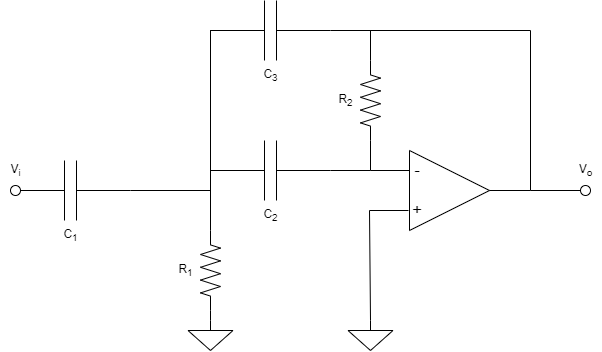
\includegraphics[width=1\textwidth]{resources/Filtro.png}
    \caption{Circuito pasa altos con retroalimentación múltiple}
\end{figure}

posee una transferencia definida
$$
    H^{*}(s) = \frac{-\frac{C_1}{C_3}s^2}{s^2+\frac{C_1+C_2+C_3}{R_2C_2C_3}s+\frac{1}{R_1R_2C_2C_3}}
$$
\vskip0.5cm

Entonces, ambas transferencias $H_1$ y $H_2$ podrán ser implementadas a partir de este circuito. Quedando entonces el siguiente filtro:
\begin{figure}[H]
    \centering
    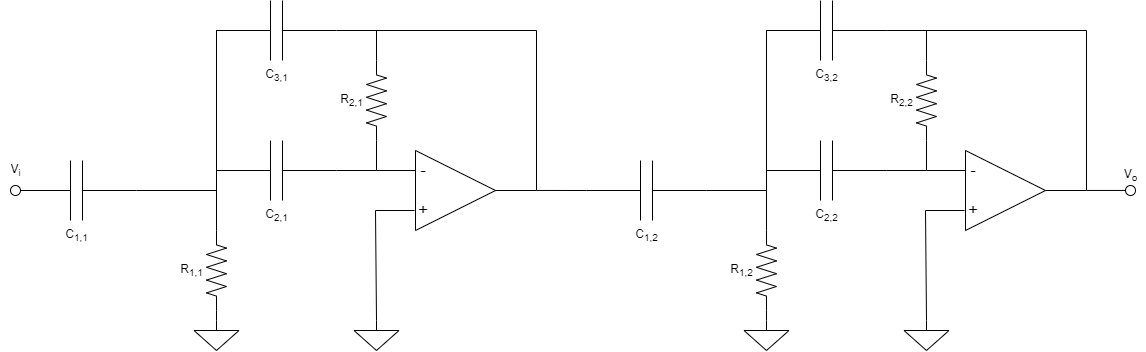
\includegraphics[width=1\textwidth]{resources/FiltroCompleto.png}
    \caption{Implementación del filtro}
\end{figure}

Siendo finalmente la transferencia:

$$
    H(s) = \frac
            {\frac{C_{1,1}C_{1,2}}{C_{3,1}C_{3,2}}s^4}
            {(s^2 +\frac{C_{1,1}+C_{2,1}+C_{3,1}}{R_{2,1}C_{2,1}C_{3,1}}s+\frac{1}{R_{1,1}R_{2,1}C_{2,1}C_{3,1}}) (s^2 +\frac{C_{1,2}+C_{2,2}+C_{3,2}}{R_{2,2}C_{2,2}C_{3,2}}s+\frac{1}{R_{1,2}R_{2,2}C_{2,2}C_{3,2}})}
$$

\hypertarget{ej4}{\section{Elección de componentes}}
Dada entonces la configuración seleccionada en la sección anterior y la transferencia del enunciado se tratará de realizar una búsqueda para los valores de los componentes que mejor se adecúen a los valores teóricos. Para ello se realizó el siguiente script en Python (cuyo objetivo es encontrar primero las posibles combinaciones de capacitores para satisfacer la ganancia y luego con ellas buscar la primera combinación de las demás resistencias y capacitores que obtengan un error relativo para los coeficientes de los denominadores menor al $5\%$) 
\lstinputlisting[language=Python]{BusquedaDeComponentes.py}

Del que se obtuvieron los siguientes valores

\begin{table}[!h]
\centering
\begin{tabular}{|c|c|c|c|}
\hline
\multicolumn{2}{|c|}{$H_{1}$} & \multicolumn{2}{c|}{$H_{2}$} \\ \hline
Componente       & Valor      & Componente      & Valor      \\ \hline
$C_{1,1}$        & 1.00n       & $C_{1,2}$       & 10n       \\ \hline
$C_{2,1}$        & 130n       & $C_{2,2}$       & 160n       \\ \hline
$C_{3,1}$        & 2.20n       & $C_{3,2}$       & 5.1n       \\ \hline
$R_{1,1}$        & 5.36k       & $R_{1,2}$       & 1.69k       \\ \hline
$R_{2,1}$        & 205k         & $R_{2,2}$       & 806k         \\ \hline
\end{tabular}
\end{table}

Con dichos valores se obtiene la siguiente transferencia:
$$
    H^{*}(s) = \frac{-0.4545s^2}{s^2 + 2271.87s + 3.18 \cdot 10^{6}} \cdot \frac{-1.9608s^2}{s^2 + 266.23s + 899680}
$$

Ya desde esta expresión podemos ver que los coeficientes de la transferencia obtenida son comparables a los coeficientes de la transferencia ideal.

\hypertarget{ej5}{\section{Cálculo del error}}
Veamos cómo se comportaron los parámetros de circuito.

\begin{table}[!h]
\centering
\begin{tabular}{|c|c|c|c|}
\hline
\textbf{Parámetro} & \textbf{Filtro ideal} & \textbf{Filtro implementado} & \textbf{Error \%} \\ \hline
K                  & 0.8911                & 0.8913                       & 0.02                       \\ \hline
$\omega_{o,1}$     & 1783.14               & 1783.85                      & 0.04                       \\ \hline
$Q_{1}$            & 0.7847                & 0.7852                       & 0.06                       \\ \hline
$\omega_{o,2}$     & 948.91                & 948.51                       & 0.04                       \\ \hline
$Q_{2}$            & 3.5583                & 3.5627                       & 0.12                        \\ \hline
\end{tabular}
\end{table}

Vemos que el circuito propuesto tiene un error prácticamente despreciable en todos los parámetros (menor a $1\%$), por lo que considero que resulta de una buena estimacíon.

Veamos cómo resultaron afectados los polos de la transferencia.

\begin{table}[!h]
\centering
\begin{tabular}{|c|c|c|c|c|c|c|}
\cline{1-3} \cline{5-7}
\textbf{$\Re$(Polo ideal)} & \textbf{$\Re$(Polo aprx)} & \textbf{Error\%} &  & \textbf{$\Im$(Polo ideal)} & \textbf{$\Im$(Polo aprx)} & \textbf{Error\%} \\ \cline{1-3} \cline{5-7} 
-1136.16                   & -1135.9                   & 0.02             &  & 1374.31                    & 1374.6                    & 0.02             \\ \cline{1-3} \cline{5-7} 
-133.34                    & -133.11                   & 0.17             &  & 939.50                     & 939.13                    & 0.04             \\ \cline{1-3} \cline{5-7} 
\end{tabular}
\end{table}

Vemos nuevamente que el error relativo, tanto la parte real como la parte imaginaria, de los polos mantiene un error relativo menor que un $1 \%$ por lo que puede ser considerado como una buena estimación.

\hypertarget{ej6}{\section{Simulaciones de la transferencia}}
En esta sección se comparará la implementación del filtro obtenida en la sección 3, que se denominará $H^{*}(s)$, con el filtro ideal $H(s)$

\subsection{Diagramas de Bode de módulo y fase}

\begin{figure}[!h]
    \centering
    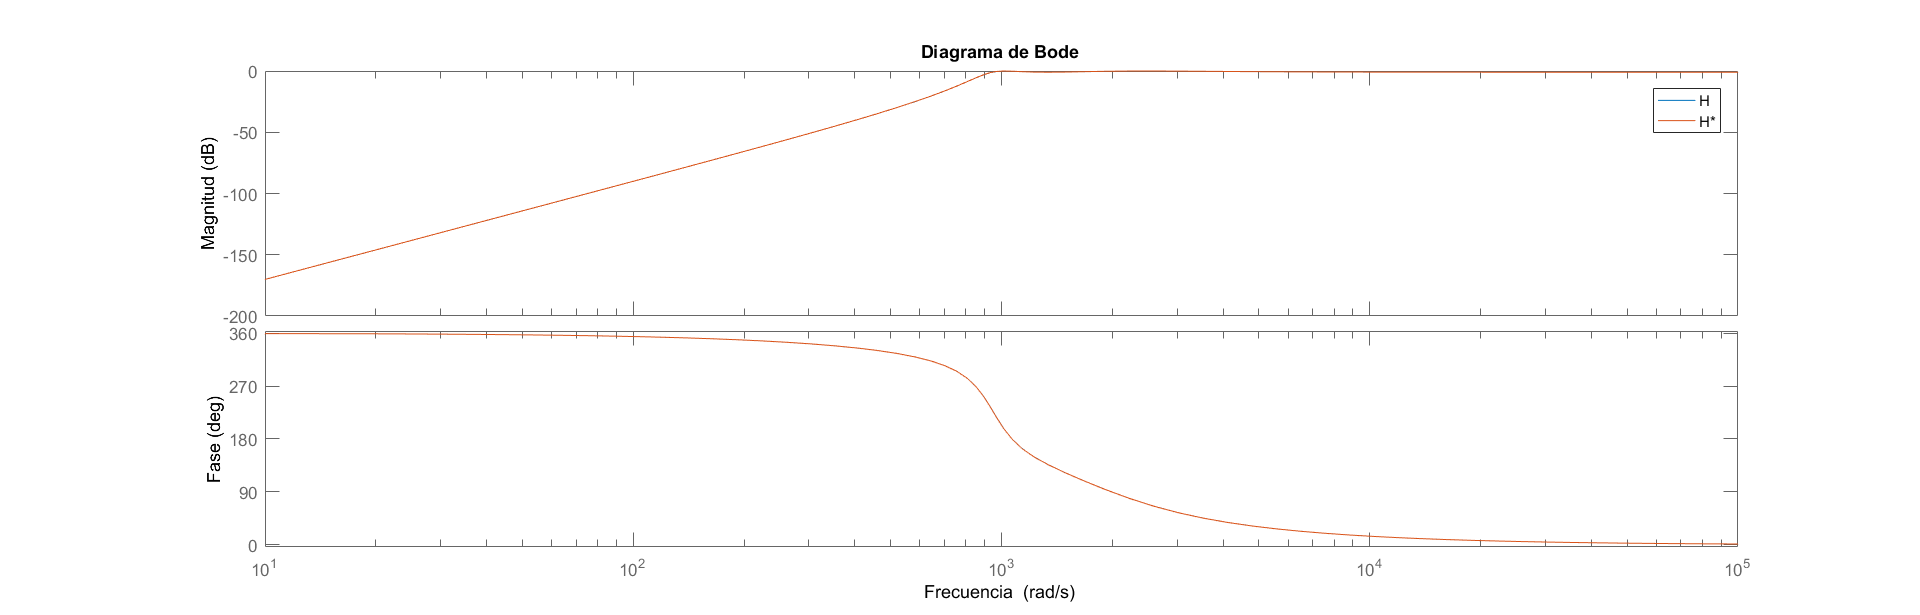
\includegraphics[width=1\textwidth]{resources/Comparacion_Bode.png}
    \caption{Comparación del diagrama de Bode}
\end{figure}

En este gráfico podemos ver que todo lo que ya fue mencionado previamente en el trabajo\\ práctico, el filtro es un pasaaltos pues para frecuencias menores a $\omega_0$ la señal se ve altamente atenuada y tendiendo a frecuencia 0 directamente se anula, mientras que para frecuencias mayores la señal se atenúa mucho menos y cuando se tiende a infinito la ganancia es constante.

\begin{figure}[!h]
    \centering
    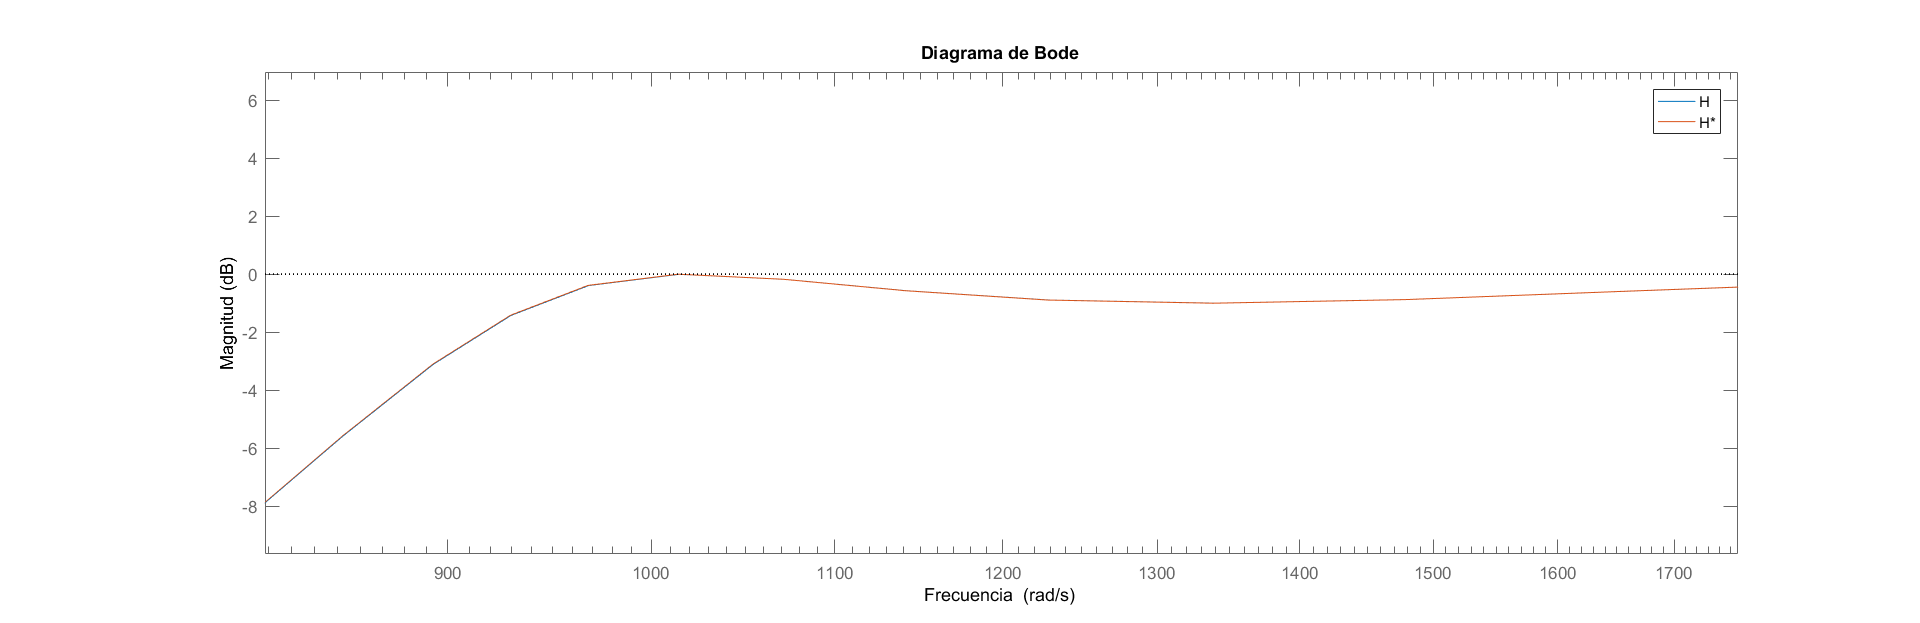
\includegraphics[width=1\textwidth]{resources/Bode_zoom.png}
    \caption{Pico en el diagrama de magnitud de Bode}
\end{figure}

En este gráfico podemos ver que efectivamente para $\omega_0 = 895 rad/s$ se alcanza $-3dB$ y luego para un valor cercano a este se alcanza un pico de $0dB$ aproximadamente en $1000 rad/s$.

Además, en este gráfico podemos ver que la diferencia entre el filtro implementado y el filtro ideal propuesto para el trabajo práctico es despreciable incluso a pequeñas escalas.

\subsection{Respuesta al escalón}
\begin{figure}[!h]
    \centering
    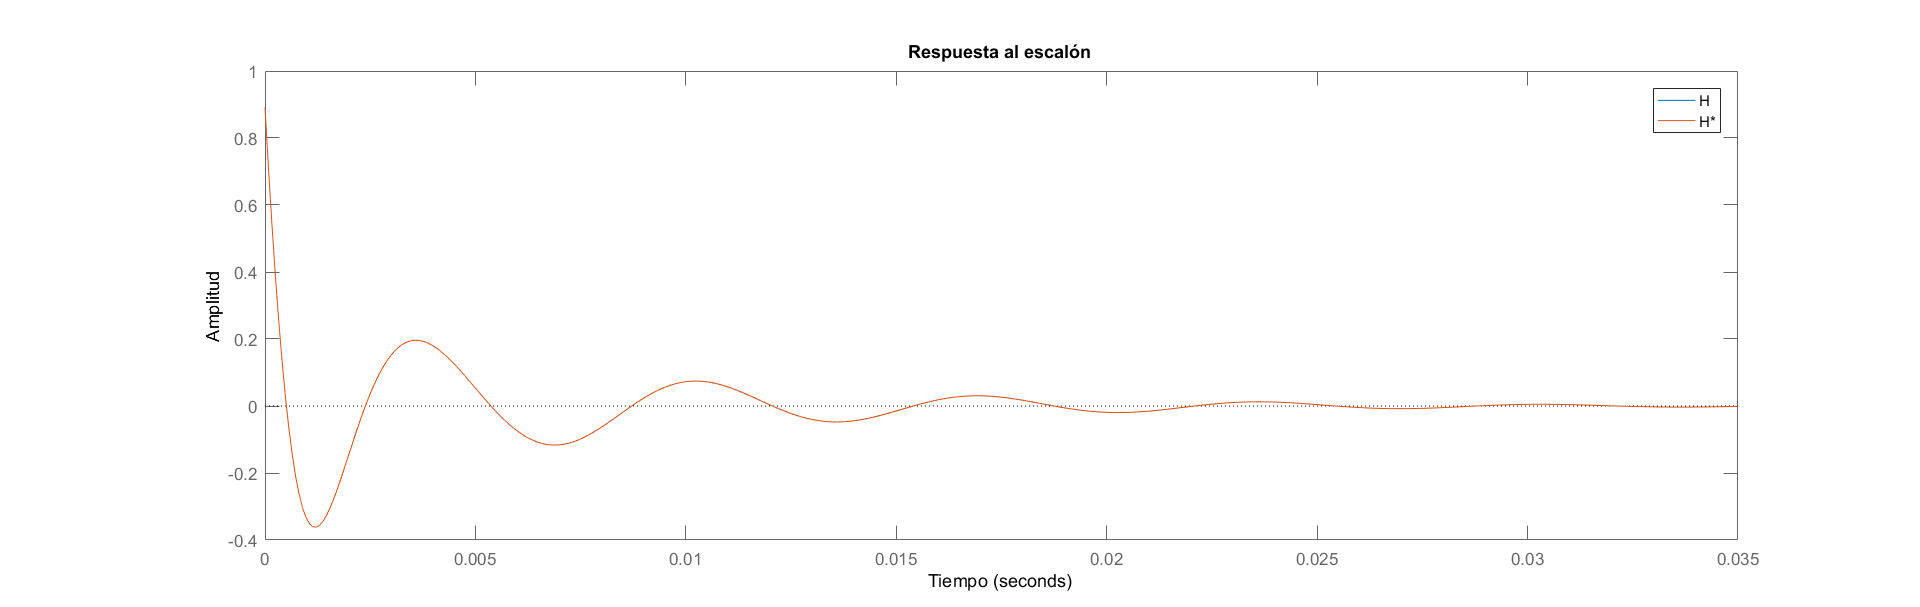
\includegraphics[width=1\textwidth]{resources/Comparacion_escalon.png}
    \caption{Comparación en respuesta al escalón}
\end{figure}

Teniendo en cuenta que la continua se trata de una señal de frecuencia cero, la señal tiende a anularse en la salida ya que como se vio en el gráfico de Bode la ganancia tiende a $-\infty$ para una frecuencia nula. La perturbación inicial se debe al comportamiento transitorio del circuito que no es tenido en cuenta para los diagramas de bode. Previamente en las secciones anteriores se había calculado, para la transferencia ideal, la respuesta analítica al escalón:

\begin{align*}
    v_o(t) & = 1.1692cos(1374.31t)e^{-1136.16t} - 0.6416sen(1374.31t)e^{-1136.16t}\\
           & + -0.2782cos(939.5t)e^{-133.34t} -0.094sen(939.5t)e^{-133.34t}
\end{align*}

De aquí obtenemos la información de los $\tau$ del circuito, estos vienen de los coeficientes que acompañan a la variable en los expontentes: $1136.16$ y $133.34$, por lo que cada coeficiente tiene asociado un $\tau_i$ respectivametente:
$$
    \tau_1 = \frac{1}{1136.16} s = 0.88ms
$$
$$
    \tau_2 = \frac{1}{133.34} s = 7.50ms
$$
Por lo que, teóricamente, el circuito estará en régimen transitorio durante $5 max(\tau_1, \tau_2) = 5 \cdot 7.50ms = 37.5ms$. Si bien dicho valor no aparece en el gráfico, se puede percibir que en un valor aproximado ($35ms$) la señal se ve atenuada por completo, que es lo que se espera en la respuesta debido a lo analizado previamente en los diagramas de Bode. 

Además agregar que como el filtro es un pasa altos podemos ver que la salida a $t=0$ es 1, y eso es porque las altas frecuencias del inicio del escalón no se ven anuladas.


\subsection{Respuesta al impulso}
\begin{figure}[H]
    \centering
    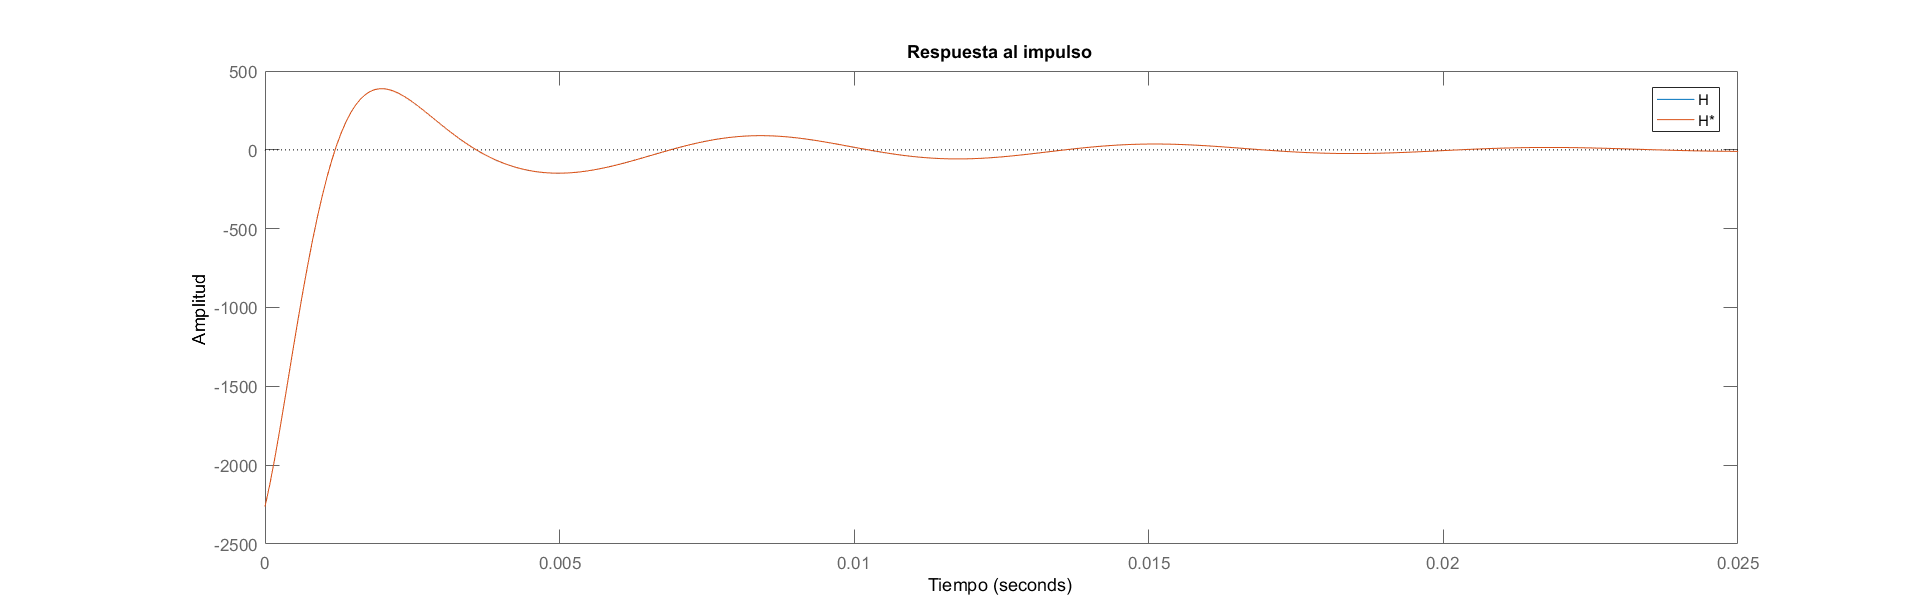
\includegraphics[width=1\textwidth]{resources/Comparacion_impulso.png}
    \caption{Comparación en respuesta al impulso}
\end{figure}
Podemos ver que, como en la respuesta al escalón, el $\tau$ es $37.5ms$, lo que se percibe en la el\\ gráfico. Prematuramente la señal alcanza valores muy negativos en la amplitud y luego crece rápidamente hasta un valor muy alto, cercano a 400 para luego tender a anularse para un tiempo cercano a $20ms$.

Como sabemos, el impulso corresponde a la derivada del escalón, y por ende se esperaba ver la misma relación entre las respuestas a ambas señales:

\begin{figure}[H]
    \centering
    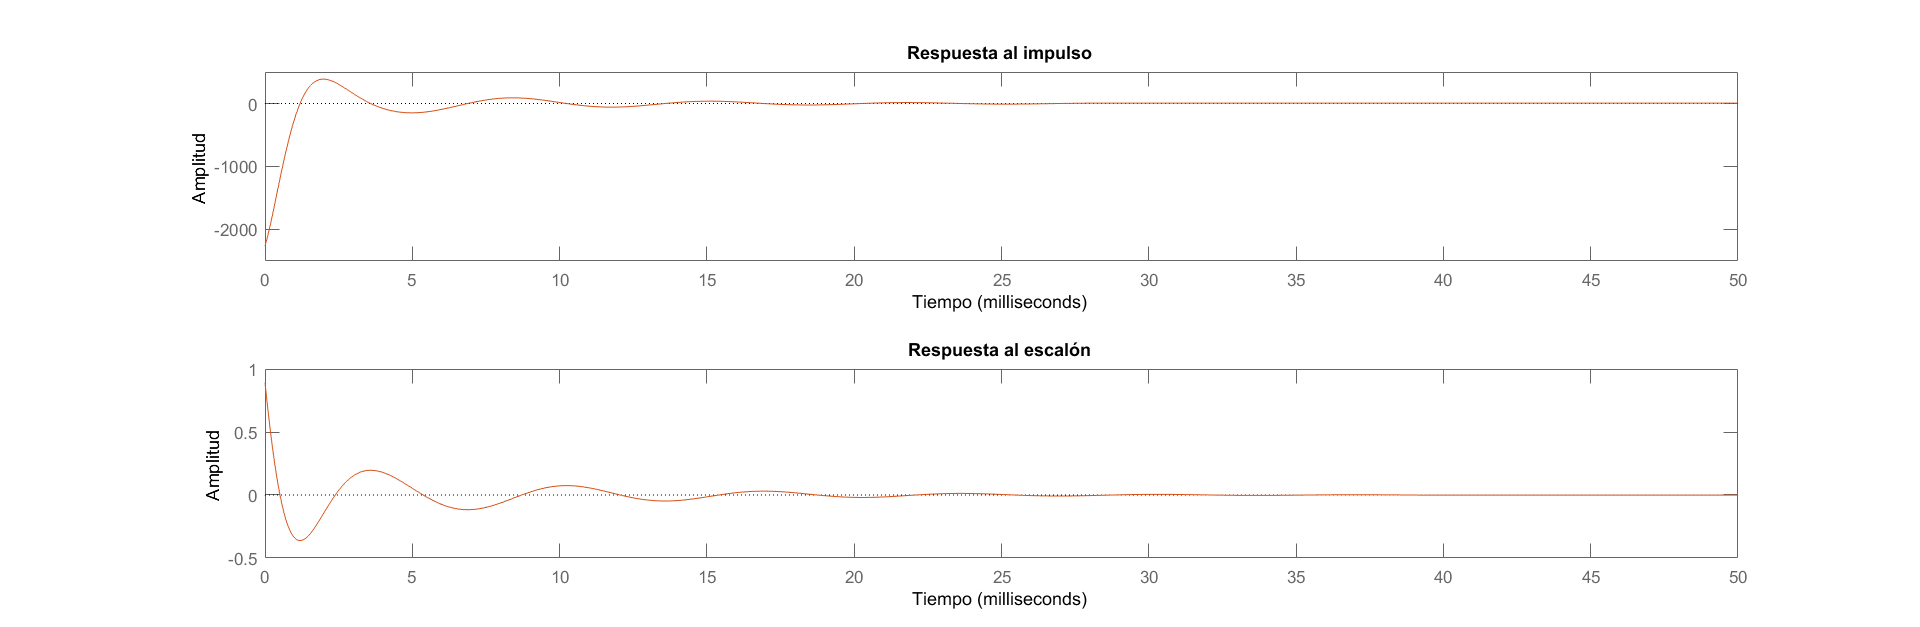
\includegraphics[width=1\textwidth]{resources/impulso_escalon.png}
    \caption{Comparación en respuesta al impulso}
\end{figure}

Comparando ambos gráficos se puede notar que cuando la respuesta al impulso se anula, la respuesta al escalón alcanza un máximo. Y además la magnitud de la respuesta al impulso se\\ puede asociar fácilmente a la tasa de cambio de la respuesta al escalón.

\subsection{Respuesta a señal senoidal}
Las frecuencias fueron elegidas para lograr entender el funcionamiento del filtro. Se escogió la frecuencia de corte de manera que se pueda ver que la señal se vea efectivamente atenuada $-3dB$ y que la fase sea aproximadamente $\pi rad$ como se vio en el diagrama de Bode. Luego se escogió $0.1 \cdot \omega_0$ para ver que la señal se vea completamente atenuada y $10 \cdot \omega_0$ para ver si la señal se atenúa aproximadamente un $10\%$ y la fase se deja intacta.

\begin{figure}[H]
    \centering
    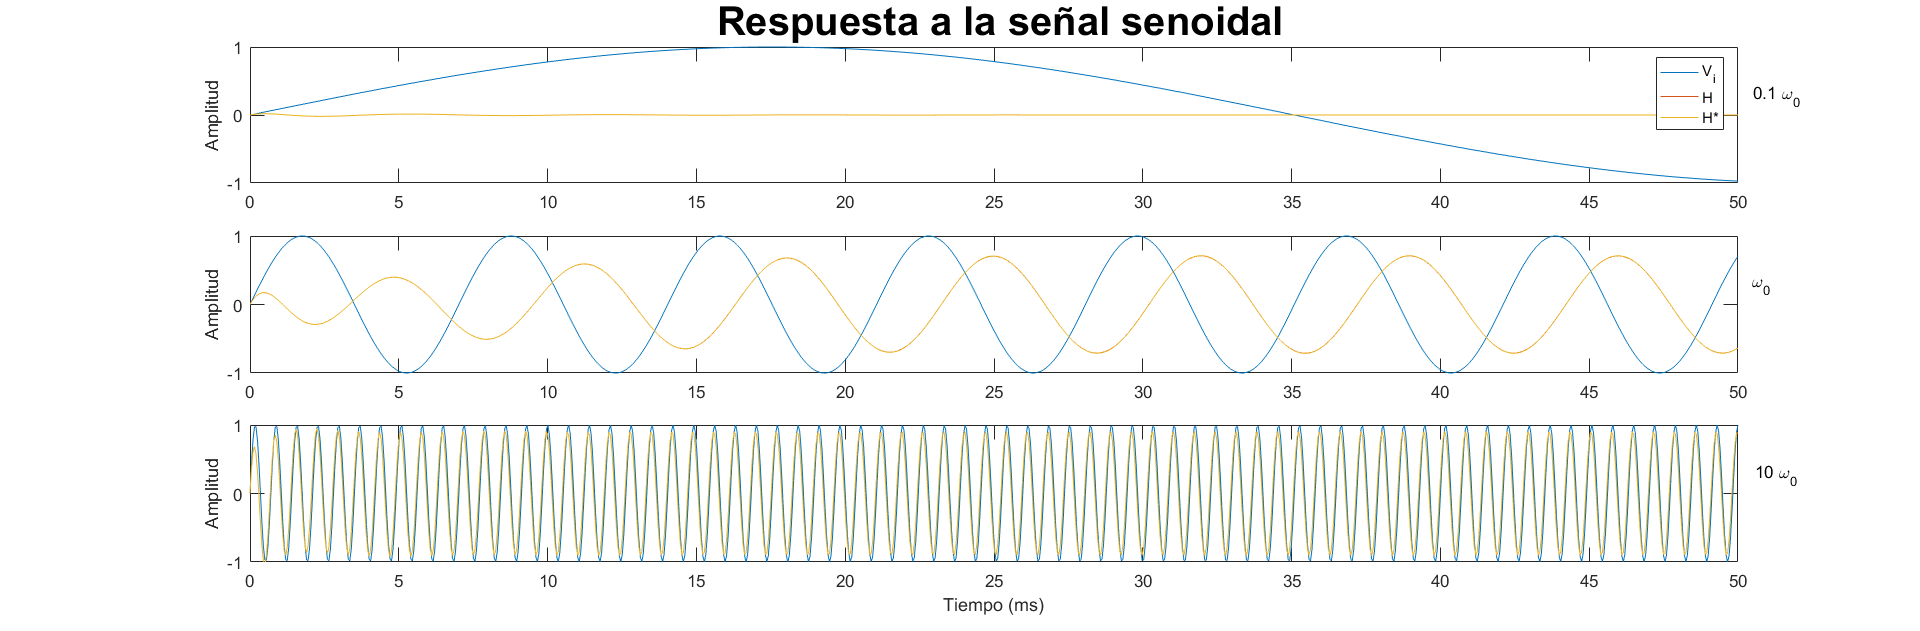
\includegraphics[width=1\textwidth]{resources/Comparacion_Seno.png}
    \caption{Comparación en respuesta a señal senoidal}
\end{figure}

Todas las premisas previamente mencionadas se vieron cumplidas en el gráfico. Podemos ver perfectamente que para el primer gráfico la señal se ve completamente atenuada, pues su frecuencia es 10 veces menor a la frecuencia de corte. Para la frecuencia de corte se puede ver que la respuesta se atenúo cerca del $30\%$ ($-3dB$) y se desfasó $\pi rad$. Luego, para 10 veces la frecuencia de corte se puede ver que la respuesta se encuentra en fase con la señal de entrada, y que además la atenuación es poca que coincide con el $10\%$ esperado.

\subsection{Respuesta a señal cuadrada}
\begin{figure}[H]
    \centering
    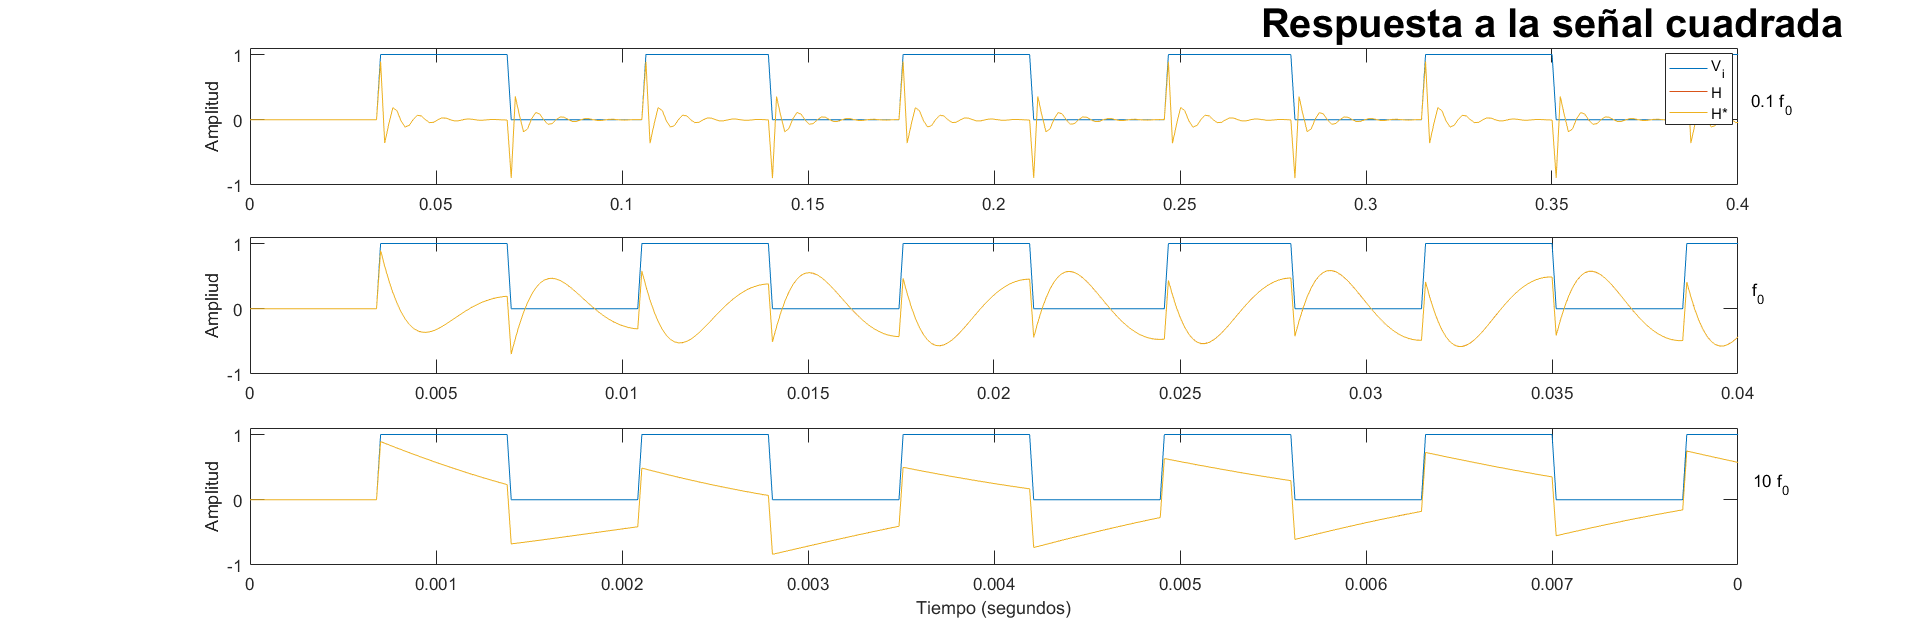
\includegraphics[width=1\textwidth]{resources/Comparacion_Cuadrada.png}
    \caption{Comparación en respuesta a señal cuadrada}
\end{figure}

Como ya se ha analizado la respuesta al escalón, es importante tenerla en cuenta para el análiis de la respuesta a la señal cuadrada, pues se trata de un tren de escalones. Hay que recordar que la respuesta al escalón tenía un $5 \cdot \tau \approx 37.5ms$.

Para el primer gráfico se puede observar que la señal está activa durante $35ms$, por lo que se puede observar que para cada activación la respuesta obtenida es similar a la del escalón.

Para el segundo gráfico la señal está activa durante $3.5ms$ por lo que no le da tiempo de atenuarse por completo, como se puede observar. Sin embargo podemos ver que la señal no se parece nada a la respuesta. Luego a medida que se va aumentando la frecuencia la señal comienza a parecerse a la señal de entrada, como ya se puede observar en el tercer gráfico donde la frecuencia es 10 veces la de corte.

\hypertarget{ej7}{\section{Simulaciones del filtro}}
\subsection{El circuito}
\begin{figure}[H]
    \centering
    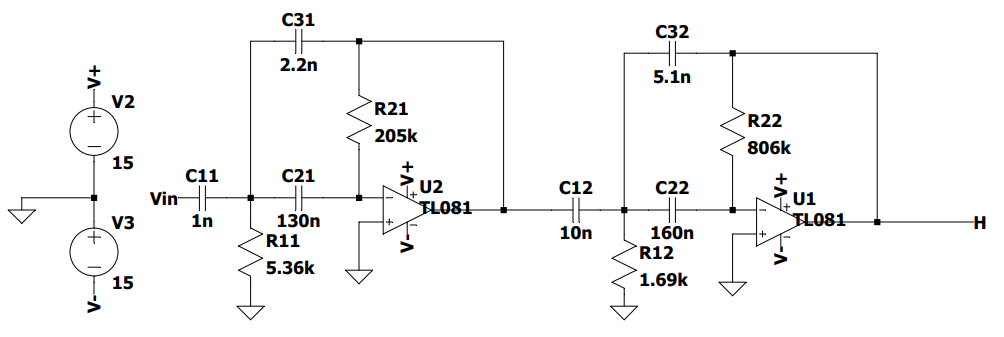
\includegraphics[width=1\textwidth]{resources/Circuito.PNG}
    \caption{Implementación del circuito en LTSpice}
\end{figure}

\subsection{Diagramas de Bode}
\begin{figure}[H]
    \centering
    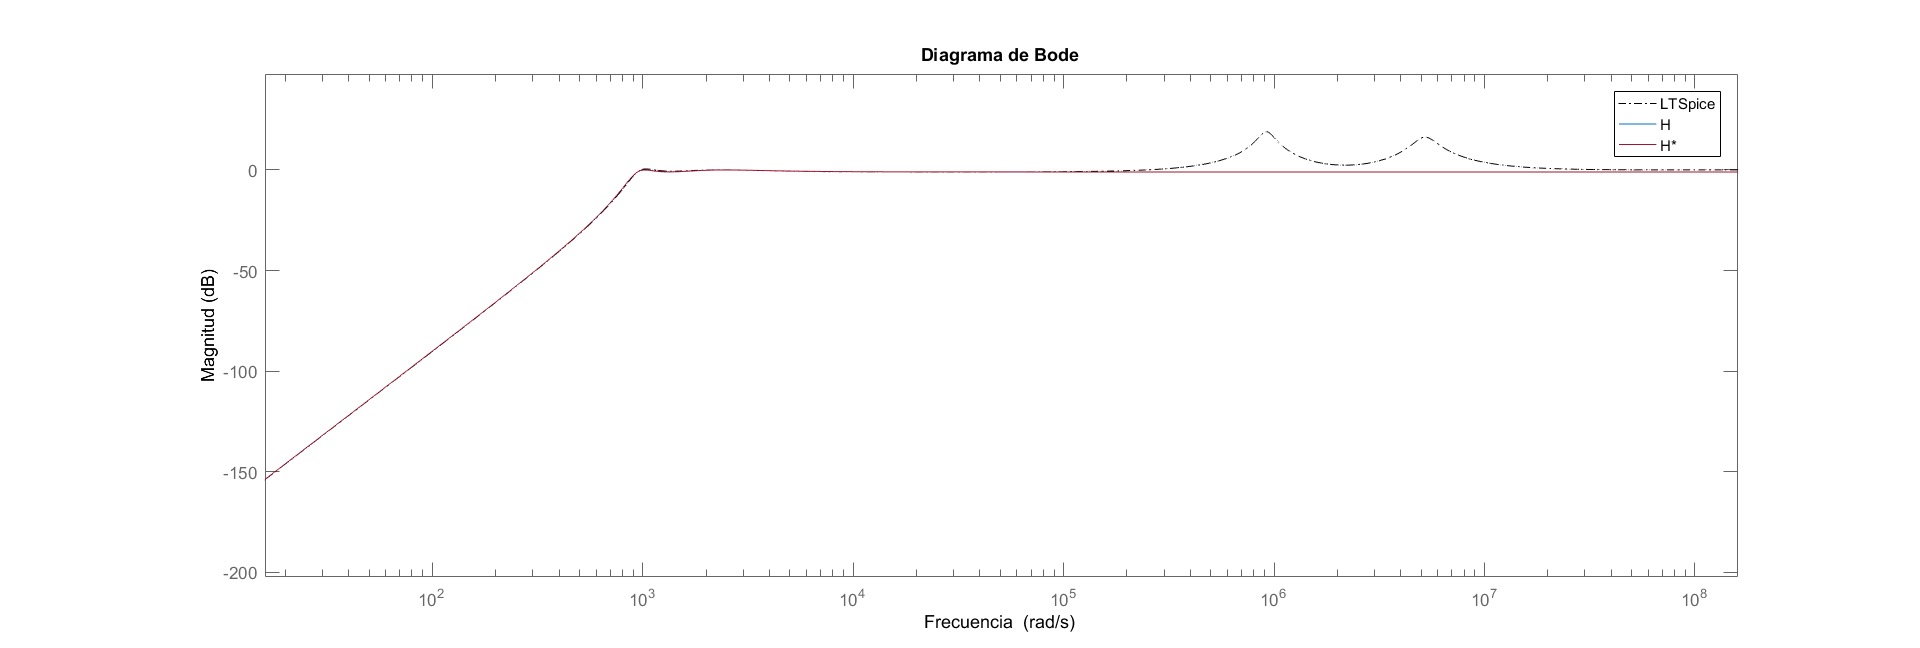
\includegraphics[width=1\textwidth]{resources/Bode_LTSpice.png}
    \caption{Diagrama de magnitud de Bode}
\end{figure}

\begin{figure}[H]
    \centering
    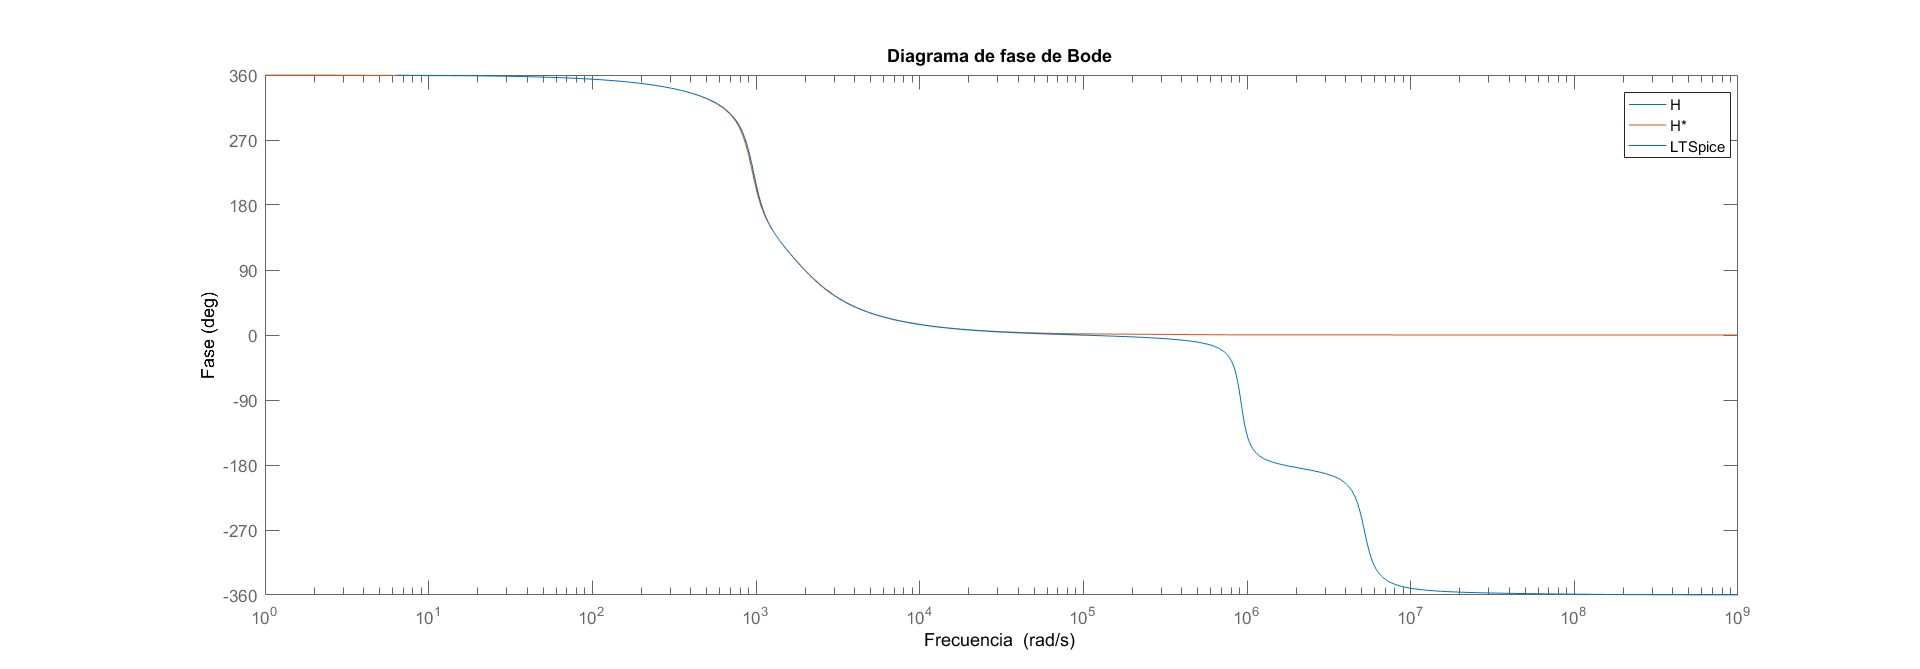
\includegraphics[width=1\textwidth]{resources/BodeFase_LTSpice.png}
    \caption{Diagrama de fase de Bode}
\end{figure}

En estos gráfico podemos ver que, a diferencia de los anteriores gráficos, aquí se puede percibir una diferencia a altas frecuencias entre lo obtenido con las simulaciones matemáticas en MatLab y lo obtenido en la simulación circuital en LTSpice. Esto se puede explicar con el uso de un modelo real para el amplificador operacional, el cual a altas frecuencias introduce nuevas singularidades al circuito que generan una diferencia en el diagrama de Bode esperado.

\subsection{Respuesta al escalón}
\begin{figure}[H]
    \centering
    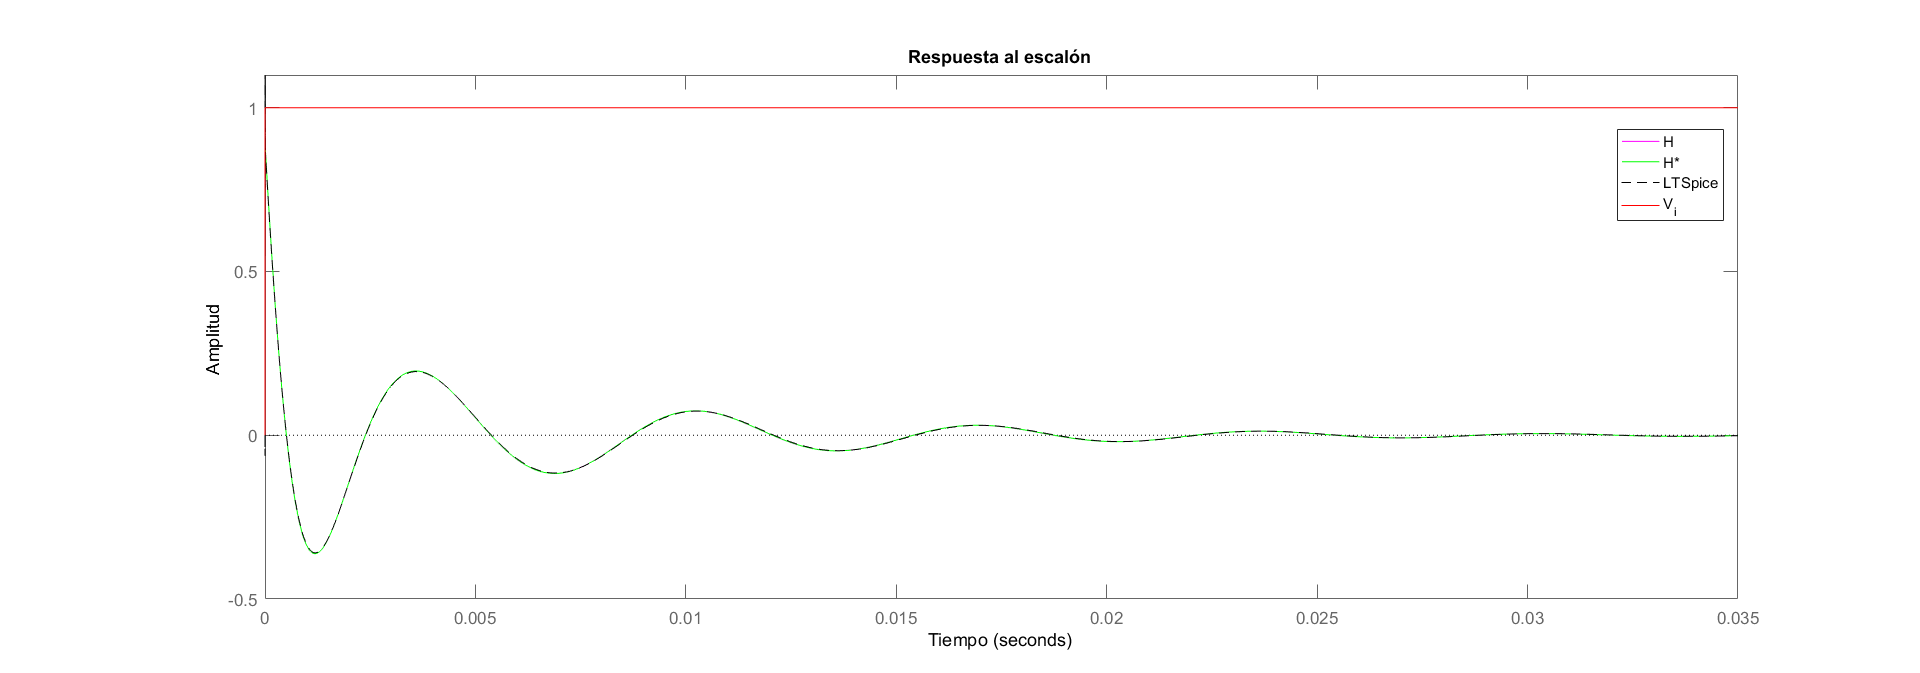
\includegraphics[width=1\textwidth]{resources/Escalon_LTSpice.png}
    \caption{Respuesta al escalón}
\end{figure}

Podemos ver en este gráfico que la señal de salida simulada con el circuito de LTSpice con el amplificador ideal es prácticamente la misma que la salida con la simulación numérica.

\subsection{Respuesta a la señal senoidal}
\begin{figure}[H]
    \centering
    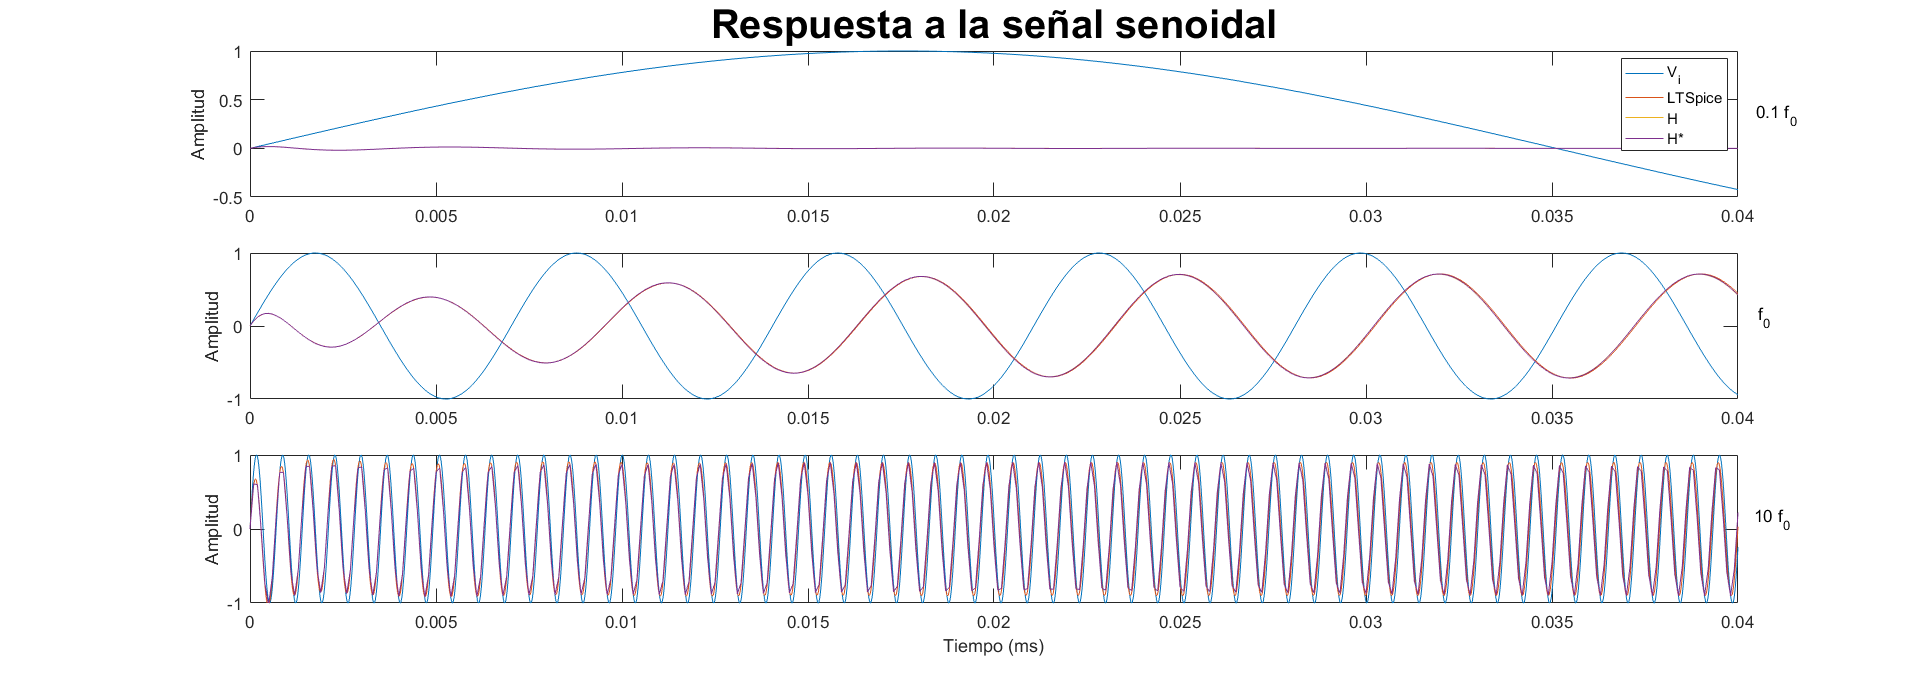
\includegraphics[width=1\textwidth]{resources/Comparacion_senoidal_LT.png}
    \caption{Respuesta a la señal senoidal}
\end{figure}
En los primeros dos gráficos no hay una difernecia significativa entre la señal de salida simulada matemáticamente y la señal de salida simulada por LTSpice con el amplificador operacional. Luego, para el tercer gráfico podemos ver que sí existe una diferencia, sobre todo en las puntas, para las señales de salida, siendo que para la salida simulada con LTSpice se obtiene una mayor ganancia que para la esperada matemáticamente. Esto podría deberse a múltiples factores.
El primer factor podría ser una discretización de la señal de salida obtenida con MatLab ya que se nota que en las puntas no parecen haber cambios suaves, sino más bien puntiagudos, y esto podría deberse a falta de muestreo por el software utilizado.
El segundo factor podría ser la alta frecuencia de la señal de entrada, como ya hemos visto en el diagrama de Bode para la magnitud, para frecuencias muy altas el circuito comienza a comportarse de forma diferente a la esperada matemáticamente ya que este modelo (el matemático) no tiene en cuenta el circuito interno del amplificador operacional real, mientras que LTSpice sí lo tiene en cuenta, de todas formas no es factible que el problema sea debido a esto último comentado, ya que para llegar a diferencias significativas la frecuencia debe ser, al menos, 2 órdenes de magnitud superior.

\subsection{Respuesta a la señal cuadrada}
\begin{figure}[H]
    \centering
    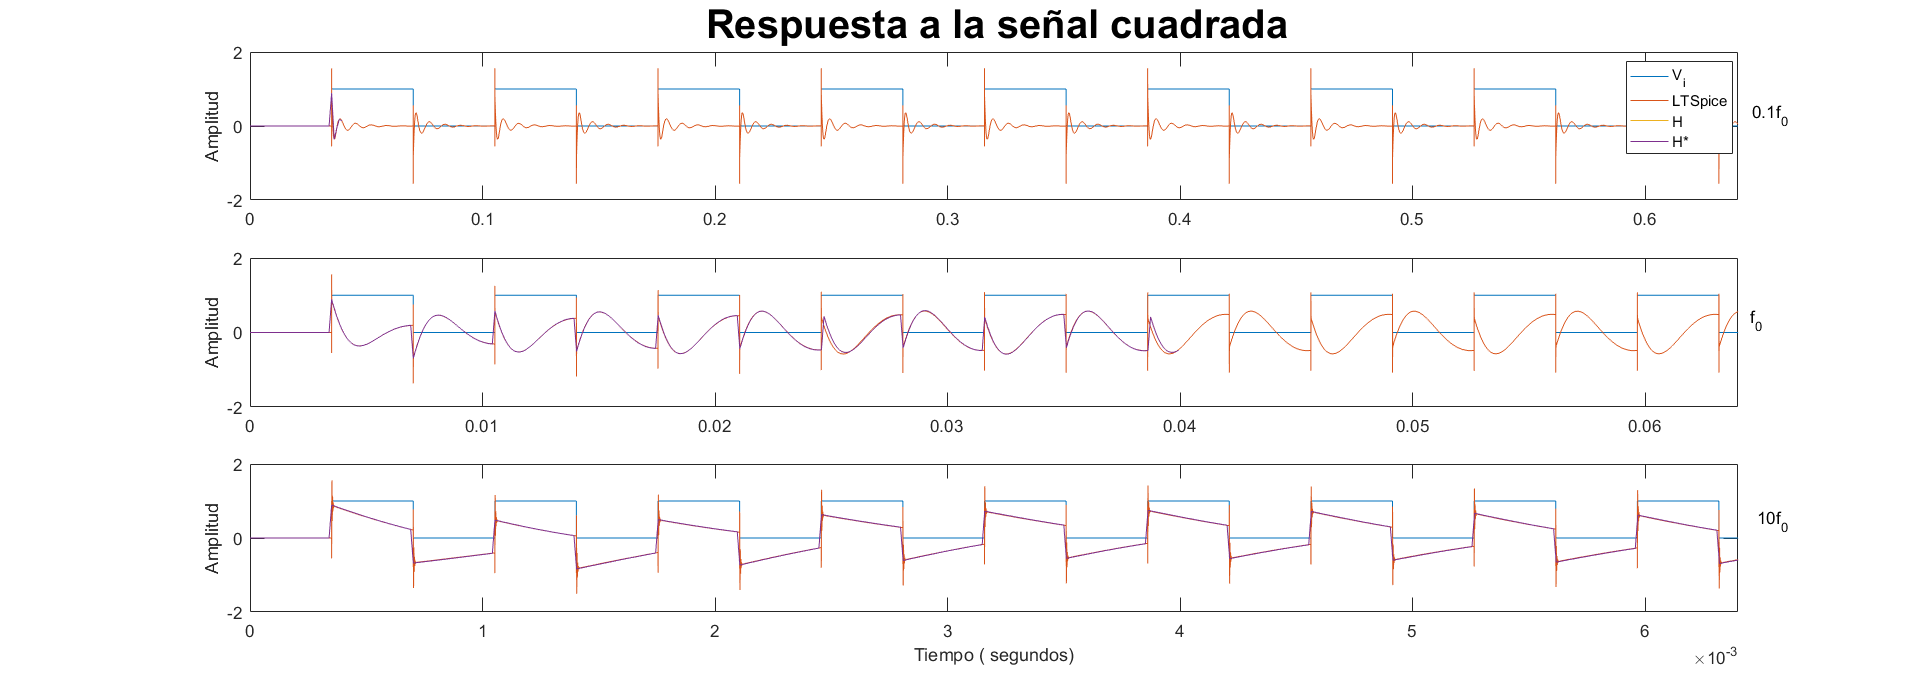
\includegraphics[width=1\textwidth]{resources/Comparacion_Cuadrada_LT.png}
    \caption{Respuesta a la cuadrada}
\end{figure}

Se puede observar que para los tres gráficos las señales de salida correspondientes a la simulación matemática y la simulación con LTSpice difieren relativamente poco. Sin embargo, la simulación de LTSpice presenta en todos los gŕaficos una diferencia en los primeros períodos  para luego estabilizarse a medida que transcurre el tiempo, estas diferencias podrían ser explicadas por las características internas del amplificador operacional.
\end{document}